
\newpage
\section{Agent-Based Foraging Model}

\subsection{Methods}
Agent-Based Models ("ABM", also known as Individual-Based Models "IBM") are a valuable tool for assessing interactions in dynamic networks like financial markets, game theory, spread of diseases or, like this case, ecosystems. The model contains multiple agents which behave independently after given behavior rules and are able to interact with the environment and each other. Agent-based models are especially suitable for analyzing behavior shifts with changing environmental conditions (eg. nectar reward or flower quantity). 

ABMs got important and popular throughout various research areas including ecology and evolutionary biology \citep{deangelis2005individual}. Also foraging models grew in number over the last years addressing a broad range of research questions. \citet{dornhaus2006benefits} looked at the benefits of a recruitment system and colony sizes. \citet{faruq2013biological} compared the foraging success while applying different flower colors by varying the wavelengths over time. \citet{bukovac2013bees} simulated the difference between the parallel visual scan of honey bees and the serial visual scan of bumble bees to for the ability to avoid distractions during foraging. The ABM of \citet{hanoteaux2013effects} showed reproduction success of plants with unequal attraction to the pollinator. 

The combination of an ABM with experimental data is a rare but promising approach. The fist to apply this method in foraging models was \citet{dyer2014bee}. They trained honey bees in a lab experiment to fine color discrimination to check for their flexibility to change when the reward changes between flower types. Afterwards, \citet{dyer2014bee} confirmed the findings with a ABM. 

I used NetLogo \citep{wilensky1999netlogo} as programming environment. It is a simple but powerful tool for making ABMs and connectible with R through the R-package "RNetLogo" \citep{thiele2014r}. 

\subsubsection*{Assumptions}

The model was developed on empirical findings for foraging rules and pollinator behavior.  It is a simple spatial model of two co-flowering plant species competing over pollination service. 

In the model, all pollinators (from now on called "bee-agents") are identical and the two flower types only differ in their initial species identity. Reward regrowth, handling times to extract the reward and its attractiveness towards the bee-agents is identical for both species. Corolla color is only assigned for better visualization and is not important for the model or the bee-agents, respectively. All bee-agents behave under the theory of flower constancy which is empirically tested and proven for various pollinators (e.g. \citet{hill1997spontaneous} for hones bees, \citet{chittka1997foraging} for bumble bees, \citet{goulson1998flower} for hoverflies and \citet{goulson1997foraging} for the butterfly \textit{Thymelicus flavus}). Flower constancy is the tendency of a pollinator to keep visiting the same flower species instead switching to more rewarding or closer species \citep{chittka1999flower,waser1986flower}. Because we are interested in the visitation rate of flowers in different frequencies, the energetic costs and the limit of gained rewards of the bee-agents are ignored. Furthermore, they do not communicate and always empty a flower completely. 


\subsubsection*{Model Environment}

In NetLogo, the "world" is a spatial grid with a set number of cells called patches. Agents are not spatially explicit and can move freely over the patches according to their given behavior rules. Patches and agents both have own properties and can interact with each other. 
In my model, the "meadow" has 100x100 grid cells with horizontally and vertically wrapping to avoid edge effects. Every grid cell can either contain a single flower of one of the two species or grass. The flowers are randomly distributed over the meadow. 
Figure~\ref{fig:cluster} gives a set of exemplary model environments with changing environmental conditions. Floral cover is defined as the percentage of the patches being flowers and the cluster number equals the average number of flowers within a flower agglomeration. Cluster can vary in the amount of flowers and shape to create a more natural meadow.

Every flower contains 1 Joule of reward in the beginning of each simulation run. The bee-agents are randomly distributed over the modeling environment, no hive is assigned and start without a fixed preference for a flower type but just pick the closest one when the simulation starts. Every tick in NetLogo equals one second. 

\subsection*{Behavior Rules}

All bee-agents act independently from each other after given foraging behavior shown in Figure~\ref{fig:flowchart} (Overview of all parameters used for the model with its default settings in the supplementary material in tab.~\ref{tab:parametervalues}).  

As mentioned in the assumptions, the behavior of the bee-agents is strongly influences by the theory of flower constancy ( e.g. \citealp{bobisud1975pollinator, chittka1997foraging, thomson1981field, chittka1999flower,  goulson1994model,  goulson1999foraging}). Bee-agents are always in favor of one of the two flowering species and forage exclusively on this species. The preference can change due to lack of searching success and a series of low rewards of the preferred flower \citep{chittka1997foraging}. Pollinators avoid recently visited flowers \citep{goulson1999foraging}. Every bee-agent is equipped with a memory to remember the location of the last four already visited flowers \citep{goulson2000pollinators}. The bee-agent can either search for a flower or visit one. 

\subsubsection*{Search}
If there is any preferred and unvisited flower in sight, the searching bee-agent moves on direct way towards the flower, otherwise it continues searching. 

Previous research on the speed of foraging pollinators by \cite{essenberg2012explaining} and \cite{kunin1991few} (in  \citealt{kunin1996pollinator}) gives 0.1m/sec as benchmark. Sequentially, bee-agents can move as fast as 1 grid cell per tick in this model. The vision of pollinators was studied in various experiments using a Y-maze apparatus \citep{dyer2008comparative, wertlen2008detection, ne2001effect}. Every bee-agent can detect flowers from a distance of 0.7m with an equivalent of 6 grid cells. The vision is reduced to a 180$^{\circ}$ cone-shaped field to the front of the agent. Pollinators tend to keep their direction while foraging \citep{waddington1980flight}. In the model, I used a correlated random walk (CRW) to achieve a relatively natural movement \citep{bartumeus2005animal, codling2008random,  pyke1992flight, viswanathan2008levy}. Empirical studies have shown a higher probability to abandon the original flower preference the longer the search remains unsuccessful \citep{chittka1997foraging}. If the bee-agent searches for 5 seconds (= 5 ticks) without finding any preferred and unvisited flower, the likelihood of changing its preference increases by 10\% with every additional tick. \\

\subsubsection*{Visit and Reward Intake}

When a bee-agent encounters a preferred and unvisited flower it takes up all its reward. The maximal reward a flower can contain is 1 Joule and refills each tick by a linear function ("reward-function", see tab.~\ref{tab:parametervalues}). The handling time involves three components: a time proportional to the amount of taken reward, a reward-independent constant and a skill factor \citep{kunin1996pollinator}. In my model, a bee-agent requires 4 seconds to extract one Joule of reward plus a reward-independent handling time of 0.5 seconds. When the bee-agent just changed its flower preference it gets a 3 second penalty for inexperience (\citealt{roubik1992ecology} in  \citealt{kunin1996pollinator}).

The reward taken is stored in the agent-own reward-memory. Every agent can remember the last four receives rewards. When visiting a flower, the bee-agent compares this memory with the current reward quantity. If the reward is less than half the average in the memory, the likelihood to abandon flower constancy and visit another species next increases by 10\%. If the reward is exceptionally good (double of there remembered average), the change probability is set to zero  \citep{chittka1997foraging, keasar1996innate}. 

The maximal number of visits within a successful pollination is possible is determined by the pollen-carryover parameter and can have a value between 1 and 16. The lower the value the stronger the heterospecific pollen interference ( \citealt{campbell1986predicting}; \citealt{benadi2012population},  \citealt{montgomery2009pollen}).

After reward-collection is completed, the bee-agent updates its flower-memory and its reward-memory and continues foraging. Each visit and successful pollination is recorded for later analysis. 


\subsection*{Simulation experiments}

Parameters altered in the main analysis are frequency, floral cover, degree of clustering and pollen-carryover rate. Each parameter-combination was run 20 times with a length of 1000 ticks each (110,400 runs in total). Additionally, I performed a sensitivity analysis with parameters which can change the behavior of the bee-agents to understand drivers of the model. Table~\ref{tab:simulation_run} presents the definition and value range of the parameters.
 

\begin{figure} [h] % screenshots
	\centering
	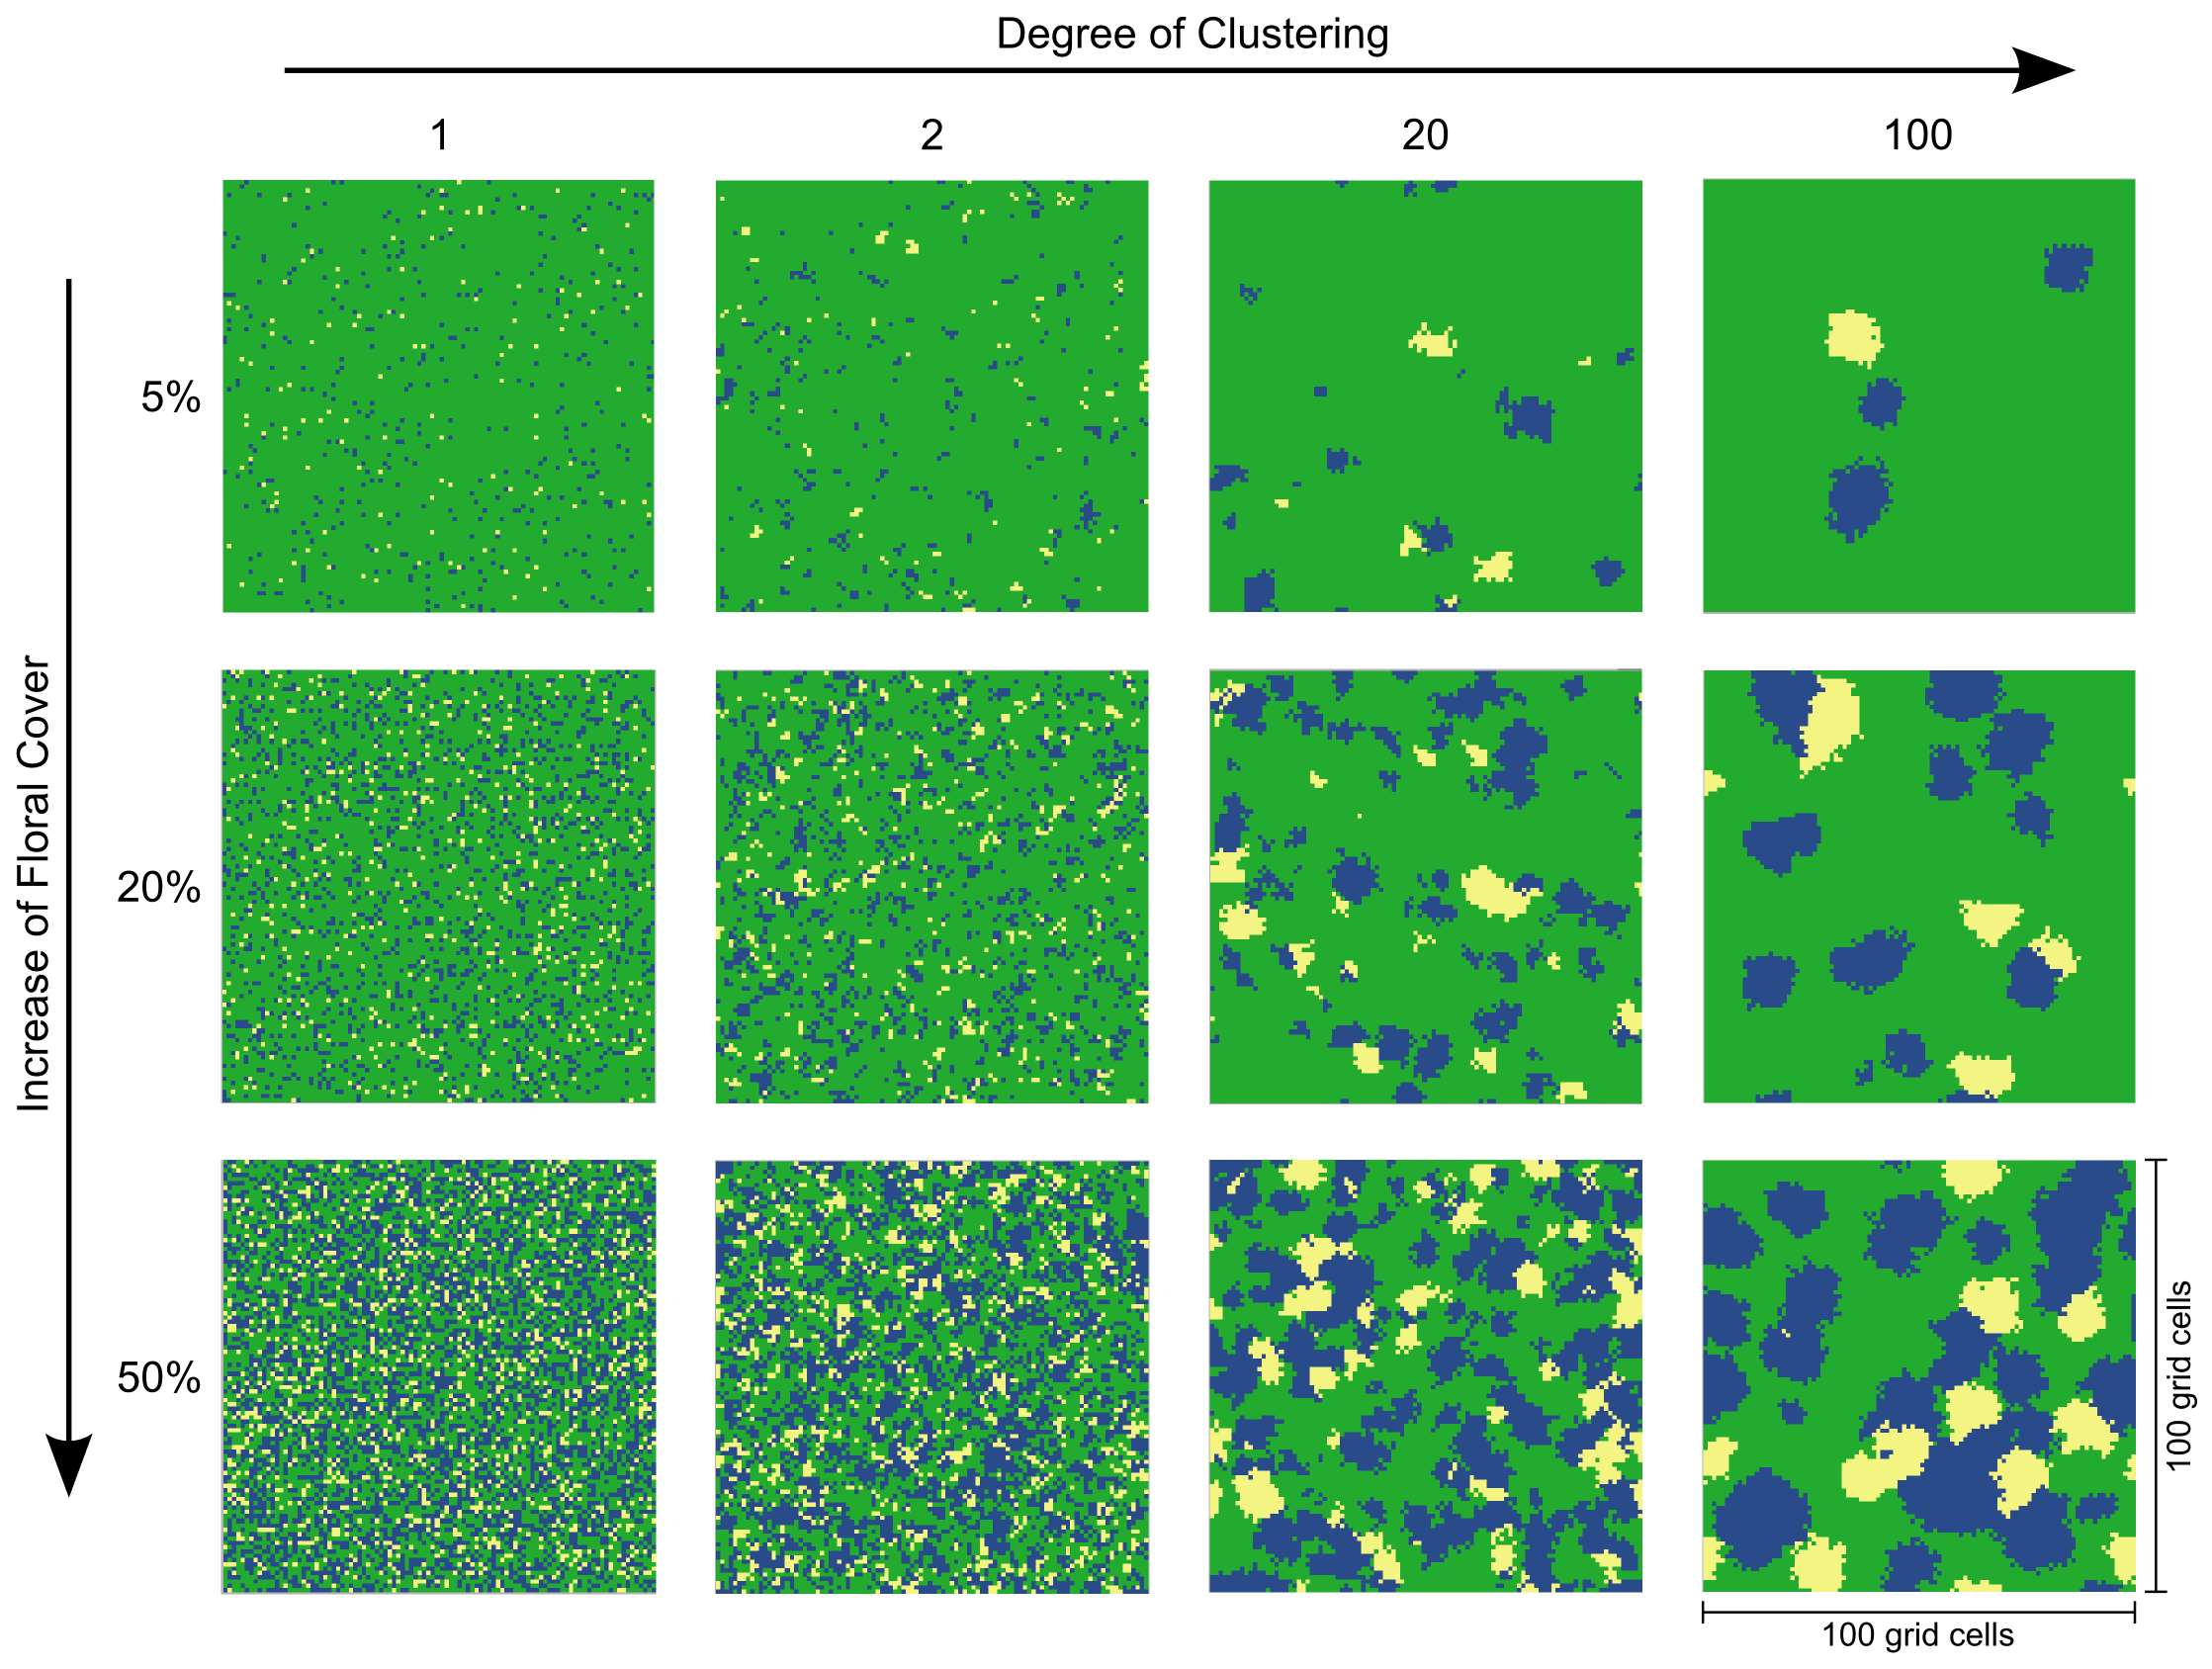
\includegraphics[width=15cm]{Images/cluster}
	\caption{ Exemplary model environment setups with increasing floral cover and degree of clustering. The cover expresses the percentage of patches containing a flower ($\Sigma_{patches}$ = 10 000). The cluster number equals the average amount of flowers per cluster. Flowers are randomly assigned to the clusters to achieve a more natural, uneven distribution. }
	\label{fig:cluster}
\end{figure}

\begin{figure} [h] %flowchart
	\centering
	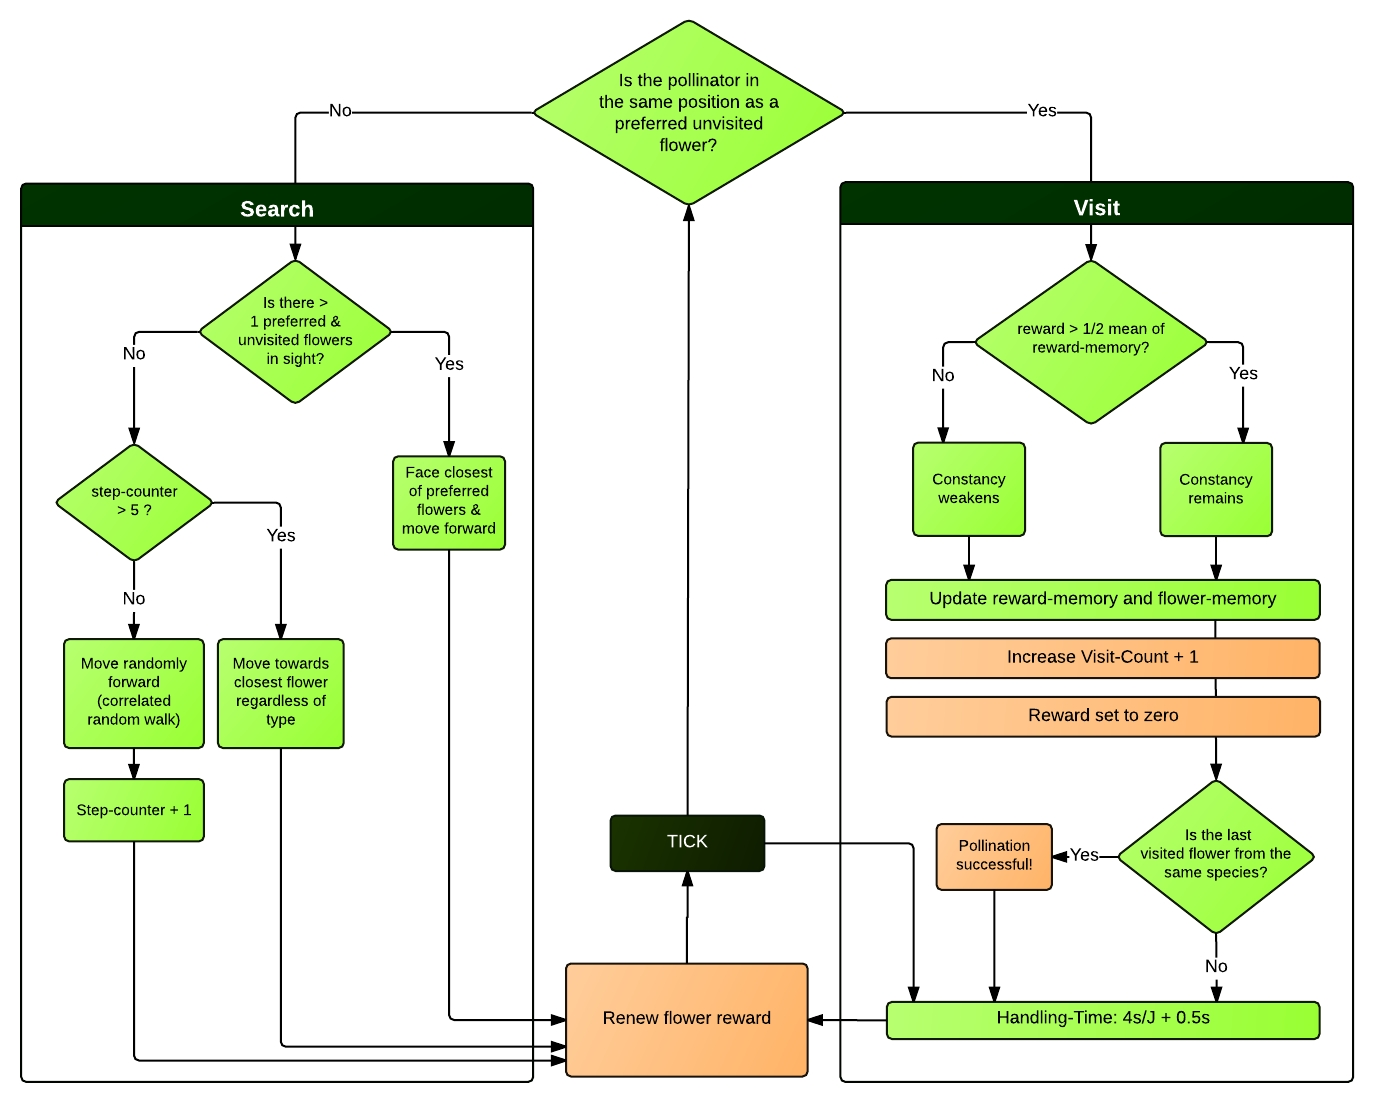
\includegraphics[width=15cm]{Images/flowchart-model}
	\caption{Flowchart describing the behavior rules for the bee-agents within the agent-based model. Every bee-agent can either search for a preferred flower or visit one. While searching, a bee-agent can remember the location of the last four visited flowers to avoid double-encountering. If there is no flower in sight after 5 seconds of correlated random walk (CRW), the probability that it will encounter the next available flower despite its type increases by 10\% per additional time step. When a bee-agent visits a flower it takes all reward within a reward-dependent handling time and compares the amount with its memory. If the reward is low, the agent is more likely to visit the other flower type next time. The maximum of visits within a successful pollination is possible is determined by the pollen carryover rate.}
	\label{fig:flowchart}
\end{figure}

\begin{table} [htbp] %parameter values
	\centering
	\caption{Parameter values used for the main and sensitivity analysis. Only general parameters were changed in the main analysis, whereas the sensitivity analysis also directly influences the behavior of the bee-agents. Within the main analysis, each combination was run 20 times for 1000 ticks (total of 110400 simulation runs) }
	\begin{tabular} {l l l}
		\toprule
		\textbf{Parameter} & \textbf{Description}  & \textbf{Values}\\
		\midrule
		\addlinespace[0.2cm]
		\multicolumn{ 3} {l} {\textsc{Main analysis}} \\ 
		\addlinespace[0.2cm]
		Frequency & Proportion of species A on all flowers  & 0-100\% (5\%-steps)\\
		Flower cover & Proportion of patches being flowers  & 5, 10, 20, 50 \%\\
		Degree of clustering & Average number of flowers per cluster   &  1, 2, 5, 10, 20, 50, 75, 100\\
		Pollen-carryover rate & Number of visits within a successful pollination is possible & 1, 2, 4, 6, 8, 16\\
		
		\addlinespace[0.2cm]
		\multicolumn{ 3 } {l} {\textsc{Sensitivity analysis}} \\ 
		\addlinespace[0.2cm]
		Reward function & Increase of reward per flower and second & 0, 0.00004, 0.001, 0.1 J/sec \\
		Vision distance & Max. range of patches within a bee-agent can detect flowers & 1, 6, 20, 50 patches\\
		Search time & \begin{tabular}{@{}l@{}} Number of seconds a bee-agent searches before\\ probability of switching flowers increases \end{tabular}   & 1, 5, 20, 50 sec \\
		Pollinator density & Number of bee-agents on the meadow & 5, 10, 20, 50 bees\\
		
		\bottomrule
	\end{tabular}
	\label{tab:simulation_run}
\end{table}


